\documentclass[12pt, titlepage]{article}
\usepackage{xcolor} % for different colour comments

%% Comments
\newif\ifcomments\commentstrue

\ifcomments
\newcommand{\authornote}[3]{\textcolor{#1}{[#3 ---#2]}}
\newcommand{\todo}[1]{\textcolor{red}{[TODO: #1]}}
\else
\newcommand{\authornote}[3]{}
\newcommand{\todo}[1]{}
\fi

\newcommand{\wss}[1]{\authornote{magenta}{SS}{#1}}
\newcommand{\ds}[1]{\authornote{blue}{DS}{#1}}

%% Graphics
\usepackage{float}
\usepackage{caption}
\usepackage{graphicx}
\usepackage{courier}
\graphicspath{ {images/} }

\begin{document}

\title{Smart Waiter Test Report} 
\author{Meraj Patel \#1137491 \\ Pavneet Jauhal \#1149311\\ Shan Perera \#1150394}
\date{\today}
\maketitle

\tableofcontents 

\listoftables

\begin{table}[H]
\section*{Revision History}
\begin{tabular}{|c|c|}
\hline
\textbf{Date}  & \textbf{Comments} \\ \hline
March 20, 2016 & Test results added \\
\hline
\end{tabular}
\caption{Revision History Table}
\end{table}

\section{Introduction}

\section{System Testing} 
\subsection{Barcode Scanning}

\subsubsection{Purpose}
Barcode scanning tests were conducted to make sure users are able to scan a barcode with minimal attempts. Also, to check if appropriate messages are displayed according to each test case.

\subsubsection{Functional Unit Test}
As per our test plan, functional unit tests were  conducted to assess test cases. Doing so replicates real world usage.

\subsubsection{Test Results}
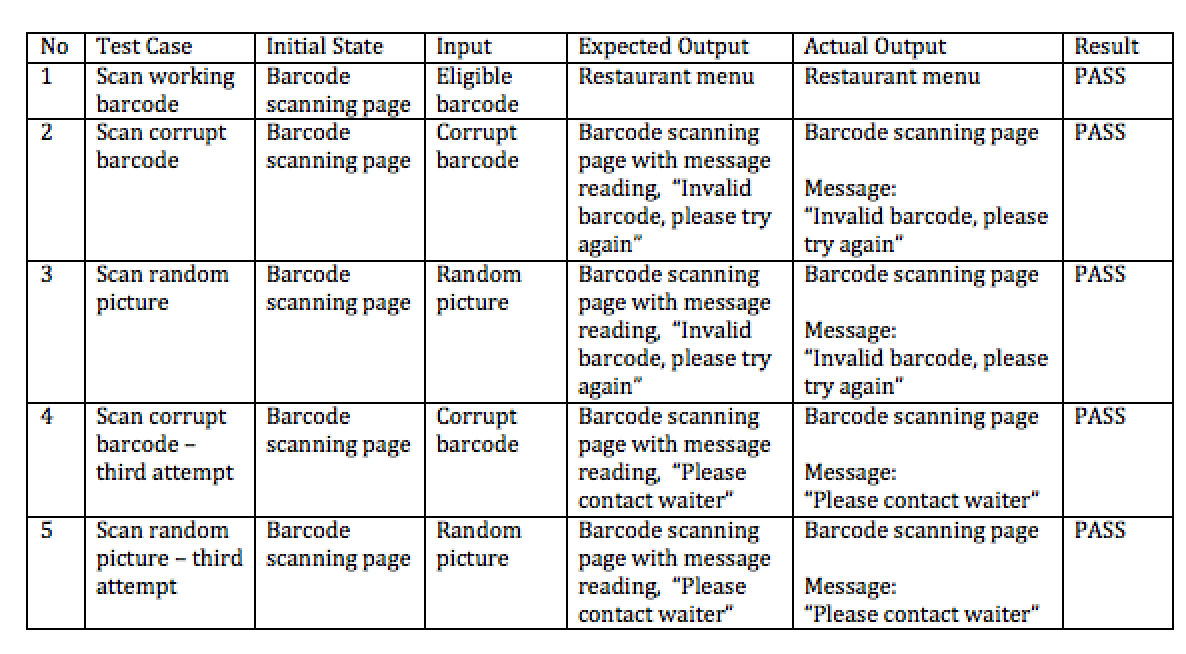
\includegraphics[width=1.2\textwidth]{barcodeTable.png}

\section{Usability Test}

\end{document}